\documentclass{article}

% Packages
\usepackage[final]{nips_2017}
\usepackage[utf8]{inputenc}
\usepackage[T1]{fontenc}
\usepackage{hyperref}
\usepackage{url}
\usepackage{amsfonts}
\usepackage{amsmath}
\usepackage{fourier}
\usepackage{graphicx}
\usepackage{wrapfig}
\usepackage{lscape}
\usepackage{rotating}

% Commands
\def\lol{\textbf{League of Legends}}
\def\version{\textbf{7.10}}
\def\champion{\mathcal{C}}
\def\ban{\champion_\mathcal{B}}
\def\available#1{\champion_\mathcal{A}^{#1}}
\def\team#1{\mathcal{T}_{#1}}
\def\win{\text{Win}}
\def\lose{\text{Lose}}
\def\rules#1#2{#1 \rightarrow #2}
\def\interest#1{\text{I}(#1)}
\def\inTplay{\text{Pl}}
\def\inTban{\text{Ba}}
\def\items{I}
\def\database{D}
\def\tree{T}
\def\node#1{T_{#1}}
\def\risk#1{R(#1)}
\def\proba#1{P(#1)}
\def\reg{\alpha}
\def\summonerItem{\mathcal{I}}
\def\summonerTrinket{\mathcal{V}}
\def\summonerSpell{\mathcal{S}}
\def\game{\mathcal{G}}

\title{Can we predict the outcome of a match in League of Legends ? Yes, we can !}

\author{
  Paul Viallard\\
  Jean Monnet University\\
  \texttt{paul.viallard@etu.univ-st-etienne.fr} \\
}

\begin{document}

\maketitle

\begin{abstract}
  After every match in \lol, a lot of statistics are provided by the game. It can be information about the game or about the players. 
  In this report, we tried to predict the winning rate of the champions which can be helpful to know the outcome of a match. 
  Secondly, we tried to predict the outcome of a ranked match. We tried different algorithms and we compared them in terms of accuracy. 
\end{abstract}

\section{Introduction}

\lol\footnote{\url{http://leagueoflegends.com/}} is a MOBA (Multiplayer Online Battle Arena) game where two teams have to compete among them. The teams are fighting in a arena where there are two team bases, some lanes and some forests called jungle.

\begin{figure}[!hb]
  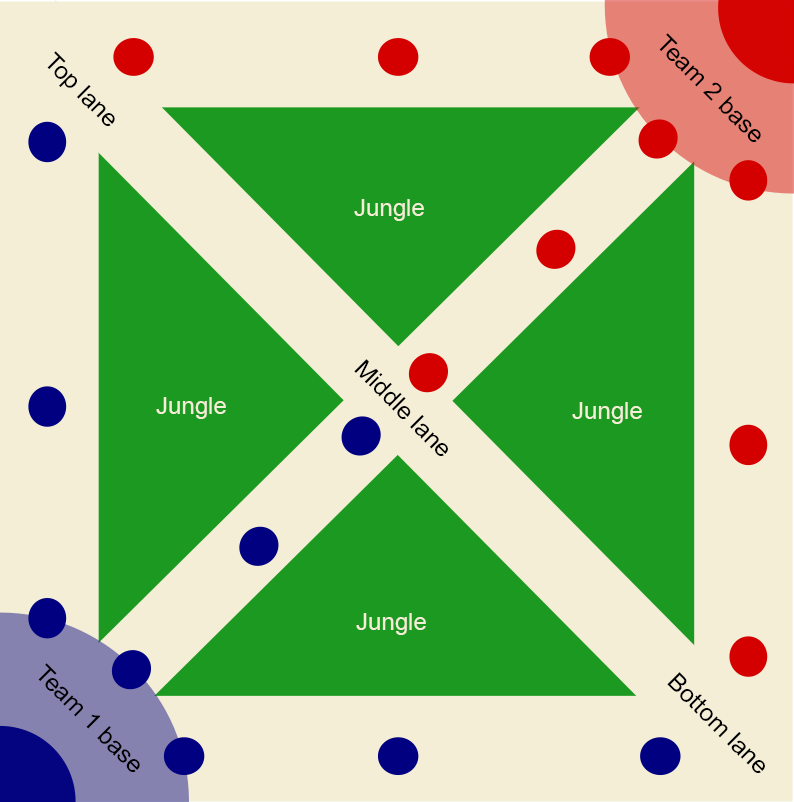
\includegraphics[scale=0.2]{map.png}
  \centering
  \caption{A typical map of a MOBA game}
\end{figure}

There are different steps before coming in the arena: the players have to ban 10 champions i.e the champions will be forbidden for the pick phase. Afterwards, there is the pick phase: this is the step where we pick the champions.\\ 
Every champion has a specific role: roughly speaking, the champion on the top has to take the damage from the enemy, the champion on the middle lane is the AP Carry (Ability Power) that is to say he must dealt magic damage to the others, the jungler has to kill the monsters in the jungle to level up, the support has to help the AD Carry (Ability Damage) in the fights on the bottom lane and the AD Carry has to kill the enemies with his physical damage. 

The first phase of the game consists in earning gold to buy items by killing the monsters. This is the time also to reach some objectives: to have the first blood (to be the first one who kill an enemy), to destroy some turrets or to kill the dragons. 
Depending on the champions and the strategies of the two teams, the second phase consists in fighting in team to finish the game. In this phase, one team finishes to kill the turrets in the enemy base and kills the nexus which marks the end of the match. 

\section{The data at our disposal}

For our study, we have 6 exported tables from Kaggle\footnote{\url{https://www.kaggle.com/paololol/league-of-legends-ranked-matches}} and two from the offical website\footnote{\url{http://ddragon.leagueoflegends.com/cdn/6.24.1/data/en_US/item.json}}\footnote{ \url{http://ddragon.leagueoflegends.com/cdn/6.24.1/data/en_US/summoner.json}} coming from the statistics that the players can see after a match of \lol. Typically, we have the total damage, the kills, the assistances, \ldots. Moreover, we have more than 50 features for the statistics of a champion and 10 features to describe the performance of the team in general.

The first table, \emph{matches}, contains the general information of the match i.e. the ID of the match, the server where the match was played, the season and the version of the game when the match was played, the date of the beginning (in timestamp) and the duration of the match.

We have a table \emph{champs} which is the list of the champions. Basically, we have an id for the champion and his name. 

For \emph{participants}, it represents the choice made during the pick phase: we have here the id of the match, the index of the player (either from 1 to 5 for the blue team or from 6 to 10 for the red team), the id of the champion which was chosen by the player, the first and second special spell chosen by the fighter, and the role of the champion (the values can be \texttt{SOLO} for the top and the middle lane, \texttt{NONE} for jungle, \texttt{DUO\_CARRY} for the AD Carry and \texttt{DUO\_SUPPORT} for the support) and finally the position of the champion (the set of values is \texttt{BOT}, \texttt{JUNGLE}, \texttt{TOP} or \texttt{MID}).

Likewise, we have a table \emph{teambans} which represent the champions banned during the pick phase. This table contains just the id of the match, the id of the team (either 100 for the blue team or 200 for the red team), the id of the champion which was banned, and the turn of the ban.

We also have the statistics of the team: the table \emph{teamstats}. The features in the table are the id of the match, the id of the team (either 100 or 200 as before), a Boolean which represents if the team had the first blood, and similarly for the first turret, the first inhibitor, the first baron, the first dragon and the first herald. Furthermore, we have the number of towers killed and similarly for the inhibitor, the baron, the dragon and the herald.

Lastly, we have a table \emph{stats} which describes the actions of a participant. We have the id of the participant, we have a Boolean which tells us if the player wins the game, there is a list of 6 items and the trinket item, the number of kills, assistances and deaths. Associated to the kills, we also have the kill performance: there is the largest killing spree which is the largest number of kills without dying, the number of killing sprees (a killing spree performance begin after 3 kills), the largest multi kill which is the number of kills performed in a short period of time and the statistics over the all types of multi kills i.e the statistics of the double kills, triple kills, quadra kills, penta kills and the legendary kills (not used in this study). The table also contains some features about damages: we have the total damage dealt and similarly with the magic, physical and true damage, we have the same features but they describe the damage dealt to the champions, we have the damage taken by our champion, the largest critical strike and also the amount of life points healed or the number of units healed. 
Moreover, we have at our disposal some general statistics about the game: there are the longest time the champion spent living, the self mitigated damage, the damage dealt to the objectives (the Dragon, the Baron, the Herald\ldots), the damage dealt to the turrets, the total time where the champion was stuck by a crowd control spell, the total crowd control time dealt by the champion, a score of the vision that the champion have during the match, the gold earned and spent to buy items, the number of turrets kills, inhibitors destroyed, the total of monsters killed, the total of neutral monsters killed, the own jungle monsters killed, the enemy jungle monsters killed, the level of the champion, the number of pink wards bought, the number of wards bought, the number of wards placed, the number of wards killed and finally a Boolean which represents if the champion had the first kill.

The data coming from the official website contains the name of the items, the name of the trinket (it is an object which permits to have a circular vision of your environment from where you're standing) and the name of the player spells.

In this study, we used the matches of the version \version. Indeed, the statistics of the champions change every version, then the statistics we did would change as well.

\section{Selecting some champions to win}

Let $\champion$ be the set of champions that are available in \lol, $\ban \subset \champion$ the set of the 10 champions banned during the ban phase (i.e $|\ban|=10$) and $\available{n} = \available{n-1}-\{c_{n-1}\}, \available{1} = \champion-\ban$ the set of champions available for the player $n$ during the pick phase.

The game use a specific order for the pick phase: alternatively, two players of a team will choose their champions. Thus, the set of champions for the teams is $\team{1} = \{c_2, c_3, c_6, c_7, c_{10}\}$ and $\team{2} = \{c_1, c_4, c_5, c_8, c_9\}$.

Before the beginning of the game, we can have an estimation of the outcome: if a champion has a bad winning rate (this is the number of games won over the number of games played) then we can estimate the outcome: we can compute the $P(\win|\team{t}'), \team{t}'\subset \team{t}$. To estimate this probability we can use the association rules, and obtain rules of the form $\rules{\team{t}'}{\{\win\}}$ or $\rules{\team{t}'}{\{\lose\}}$ and use the confidence.

To mine with the association rules, we created a database $\database$ composed of $m$ games with the items $\items=\champion\cup\{\win,\lose\}$ and $\database = \{\team{w}^{(1)}, \team{l}^{(1)},\dots, \team{w}^{(m)}, \team{l}^{(m)}\}$, where $\team{w}^{(k)}=\team{i}^{(k)}\cup\{\win\}$ is the transaction which represents the team $i$ which won the match $k$ and $\team{l}^{(k)}=\team{j}^{(k)}\cup\{\lose\}$ the team $j$ which lost the match $k$. 

After computing the following results with the Apriori algorithm, we obtained some interesting rules: first of all, we got the win rate of the champions. Indeed, we had some rules of the form $\rules{\{c\}}{\{\win\}}$ or $\rules{\{c\}}{\{\lose\}}$ with $c\in\champion$. Secondly, we obtained some rules with a combination of champions in the right part and either $\win$ or $\lose$ in the left side i.e $\rules{\champion'}{\{\win\}}$ or $\rules{\champion'}{\{\lose\}}$ with $\champion'\subset\champion$. As we can notice, these rules are also interesting because we can know if a combination of champions (especially in the bot lane) is strong in a particular version.

For the version \version, the following are examples of interesting rules:
\begin{verbatim}
    {Ryze}          => {Lose}   confidence: 0.6298434
    {Ahri,Janna}    => {Win}    confidence: 0.5942783
    {Caitlyn,Janna} => {Win}    confidence: 0.5479134
\end{verbatim}
We can remark that Ryze is not the champion to play in this version ... Indeed, the win rate is 37.02\% which is very low.
Furthermore, we had some rules with champions of different lanes: Janna is a support and Ahri is an AP Carry who is played at the middle lane. Thus, we guessed that the pair can be efficient in the team fights for example. After, we had rules with two champions in the same lane: the bottom lane. We can deduce that the two are good together in the lane phase of the game.

It can be interesting if we look at the interest that a player can have to the champions. We defined the interest of a champion as $\interest{c}=\inTplay(c)+\inTban(c)$ where $c\in\champion$, $\inTplay$ is a function of $c$ which produce the frequency of choosing the champion and $\inTban$ is a function of $c$ which produce the frequency of banning the champion. We plotted the interest of a champion in the Figure~\ref{fig:freq}. Obviously, we can see that Ryze is not very interesting for the players or that Ahri is picked or banned a lot which is consistent with the previous results.

\section{Using some items}

We conduct another study on the items: indeed, it can be interesting to observe if there are some strong item for a particular version. Moreover, the statistics of the items is also regularly up to date which means that some items can be very strong for a certain amount of time.\\ 

Let $\summonerSpell$ the set of player spells which is available in \lol. It is composed of 12 elements i.e $\summonerSpell = \{\text{Barrier}, \text{Clarity}, \text{Cleanse}, \text{Exhaust}, \text{Flash}, \text{Ghost}, \text{Heal}, \text{Ignite}, \text{Mark}, \text{Dash}, \text{Smite}\\, \text{Teleport}\}$. During the pick phase, a player $j\in\left[1,10\right]$ has to take 2 different spells $s_{1,j}\in\summonerSpell$, $s_{2,j}\in\summonerSpell$ which can be useful later during the match. 
Furthermore, in the game, the player $j$ can take a trinket $t_j\in \summonerTrinket$ and 6 items $i_{1,j},\dots, i_{6,j}\in \summonerItem$ where $\summonerTrinket$ is the set of trinkets and $\summonerItem$ the set of item provide by \lol. 
Let $f_{j}$ the function which return the outcome of the match for the player $j$. 

We created a database $\database$ composed of $m$ games where $\database=\{\game^{(1)}_1\dots\game^{(m)}_{10}\}$ and $\game^{(k)}_{j}=\{c_j^{(k)}, t_j^{(k)}, i_{1,j}^{(k)},\dots, i_{6,j}^{(k)}, s_{1,j}^{(k)}, s_{2,j}^{(k)}, f_j^{(k)}\}$ is the statistics of the game $k$ for the player $j$.

We obtained the following results:

\begin{verbatim}
    {item6=Rabadon's Deathcap}  => {win=Win}    confidence: 0.6549605
    {item6=Guardian Angel}      => {win=Win}    confidence: 0.6458249
    {item5=Ardent Censer}       => {win=Win}    confidence: 0.6312394
    {item5=The Bloodthirster}   => {win=Win}    confidence: 0.6301214
\end{verbatim}

The rules are interesting because we can see a winning rate for some items. In the version \version, we can see that some items are very strong: for example the Gardian Angel has a win rate of 64.58\% when it is used as last item.

\section{Predicting the outcome}
To predict the outcome of a match, we will now consider only the statistics of the match i.e the algorithms will not use the pick phase information. We constructed a new dataset $\database$ constituted only by numeric values. Let define the new dataset as $\database=\{(x^{(i)}, y^{(i)})\}_{i=1}^{m}$ where $m$ is the number of game.\\ 
We changed the label of the original dataset: $y^{(i)}$ is now a Boolean which represent the outcome of the team 1 that is to say $y^{(i)}=0$ if and only if the team 2 win and $y^{(i)}=1$ otherwise.

Moreover, $x^{(i)}=x_{\mathcal{G}}^{(i)}.x_{\mathcal{T}1}^{(i)}.x_{\mathcal{T}2}^{(i)}$ is now a huge vector which contains the information of the game $x_{\mathcal{G}}^{(i)}$, the information about the team 1 $x_{\mathcal{T}1}^{(i)}$ and about the team 2 $x_{\mathcal{T}2}^{(i)}$. Typically, $x_{\mathcal{G}}^{(i)}$ contains the information that we have in \emph{matches} and $x_{\mathcal{T}j}^{(i)}$ contains the information that we have in the tables \emph{teamstats} and \emph{stats}. The vector $x_{\mathcal{T}j}^{(i)}$ for the team $j$ in the game $i$ can also be decomposed in several parts: firstly, it contains the information in the table \emph{teamstats} and then we have the features of the table \emph{stats} for each champion which plays in the team $j$.

\subsection{Visualizing the data}

Given the fact that the dimension of $x^{(i)}$ is huge, we can reduce the dimension of the data to visualize how the data points are located in the space. We obtained something interesting with a PCA: in 2D, we can see that the ''majority'' of games labeled 0 are in the lower part of the graph and the games labeled 1 are in the upper part of the plot. Actually, as we can see in the Figure~\ref{fig:vectors}, the vectors  of the total damage dealt by the AD Carry split the space in 2: it projected the example where the given team win in the direction of the vector of the total damage dealt.  Indeed, this type of champions has to do physical damage to kill the champions of the other team. Obviously, here the vectors of the physical damage dealt by the AD Carry is near the previous described vector. However, the representation is not representative of the true space: the first three principal components explain just 53.33\% of the variance.

\begin{figure}[!tbp]
  \centering
  \begin{minipage}[b]{0.4\textwidth}
    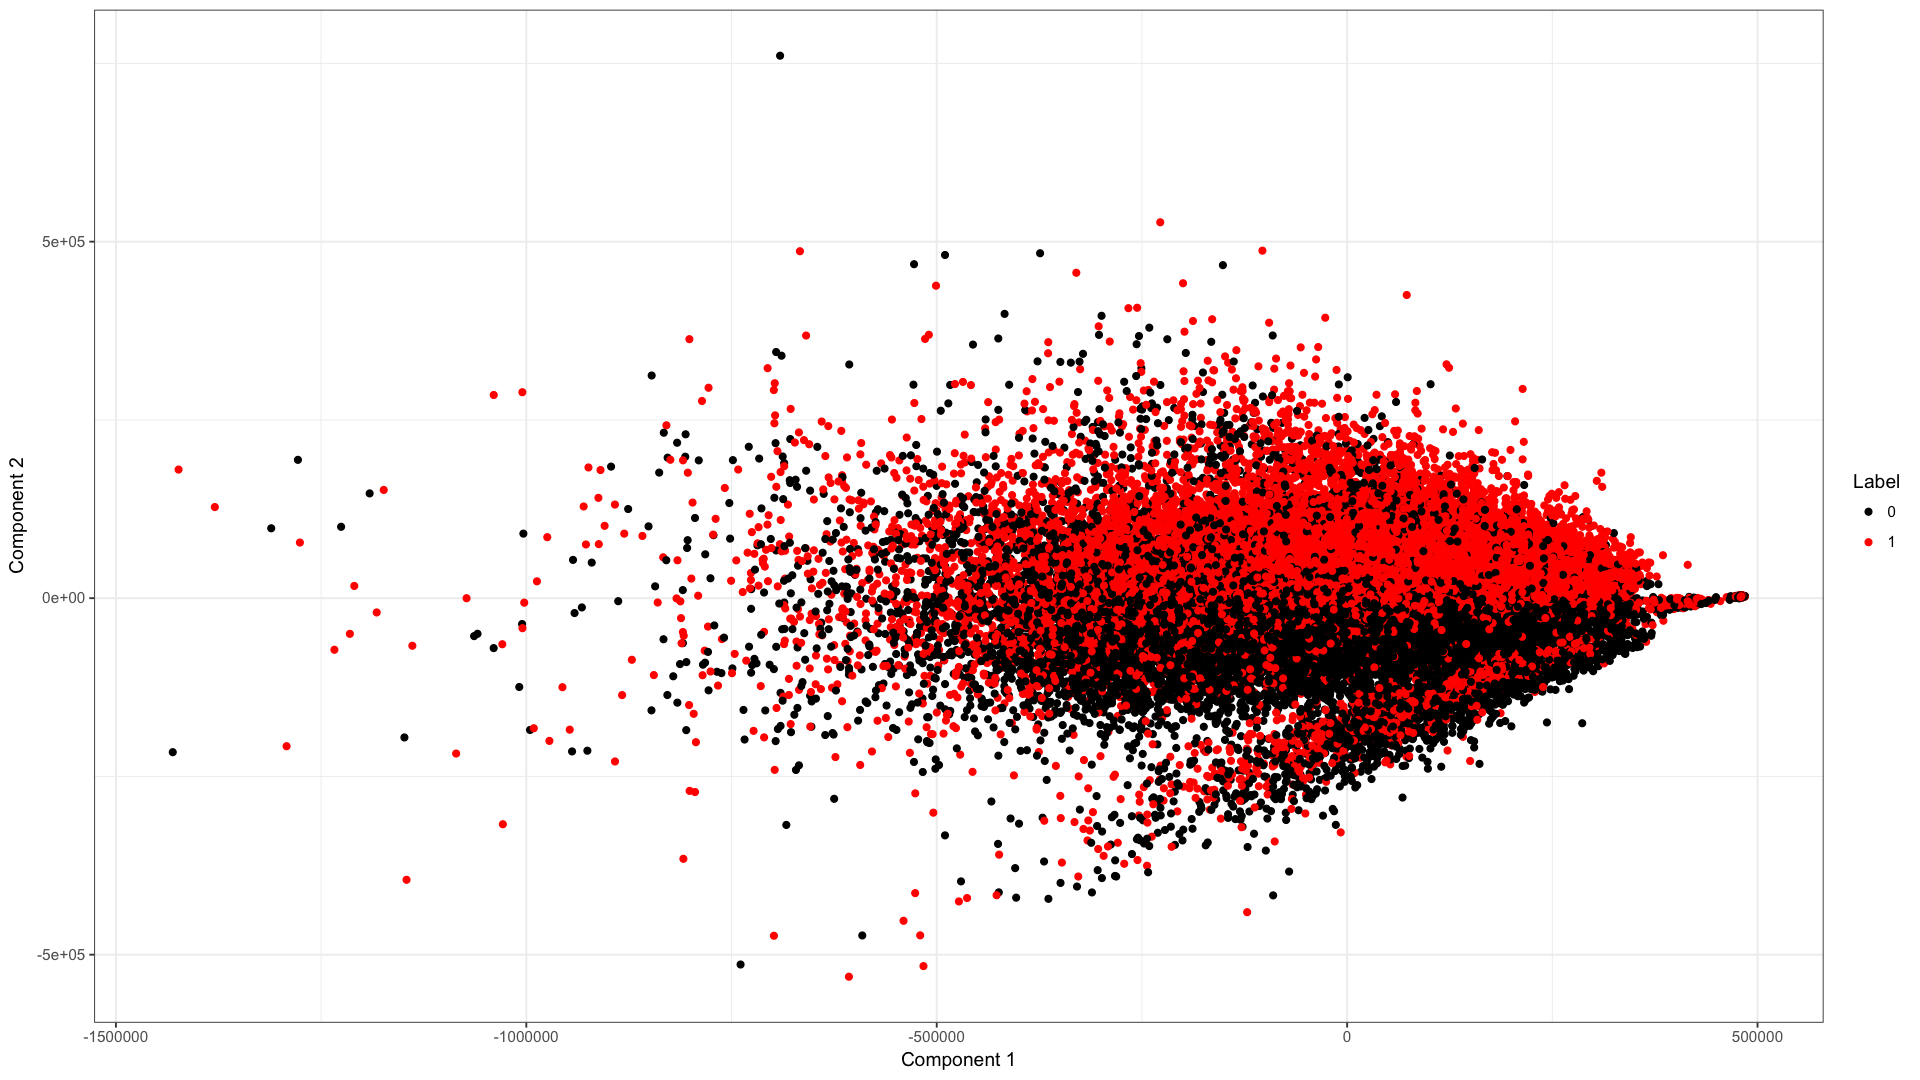
\includegraphics[width=\textwidth]{PCA1.png}
    \caption{The data in 2D}
  \end{minipage}
  \hfill
  \begin{minipage}[b]{0.4\textwidth}
    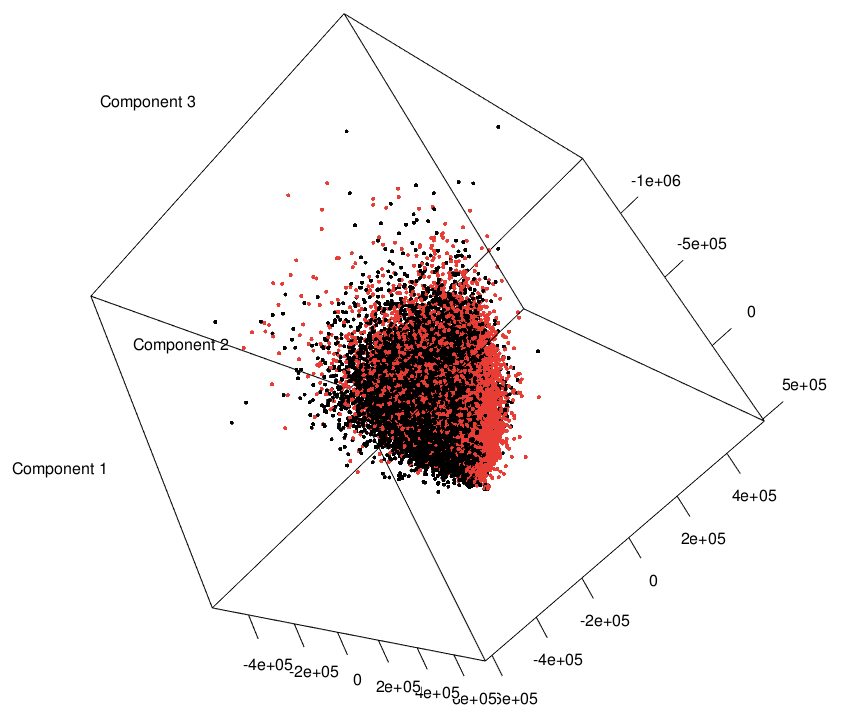
\includegraphics[width=\textwidth]{PCA2.png}
    \caption{The data in 3D}
  \end{minipage}
\end{figure}
\subsection{Inferring some decision trees}

We inferred a decision tree with the entropy and one with the gini index. For the two trees, the parameters has the default values i.e  the minimum of splits is set to 2 and the minimum of buckets is set to 1. However, we used a grid search to set the complexity $\reg$ of the tree. Indeed, let $\node{1},\dots,\node{k}$ be the nodes of the tree $\tree$. If we want to minimize the risk at test time of the tree $\risk{\tree}=\sum_{i=1}^{k}\proba{\node{i}}\risk{\node{i}}$, we have no regularization here which can lead to over-fitting. For this reason, we add a regularization term $\reg$: $\risk{\tree_{\reg}} = \risk{\tree}+ \reg|T|$ where $|T|$ is the size of the tree. 

\begin{figure}[!hb]
  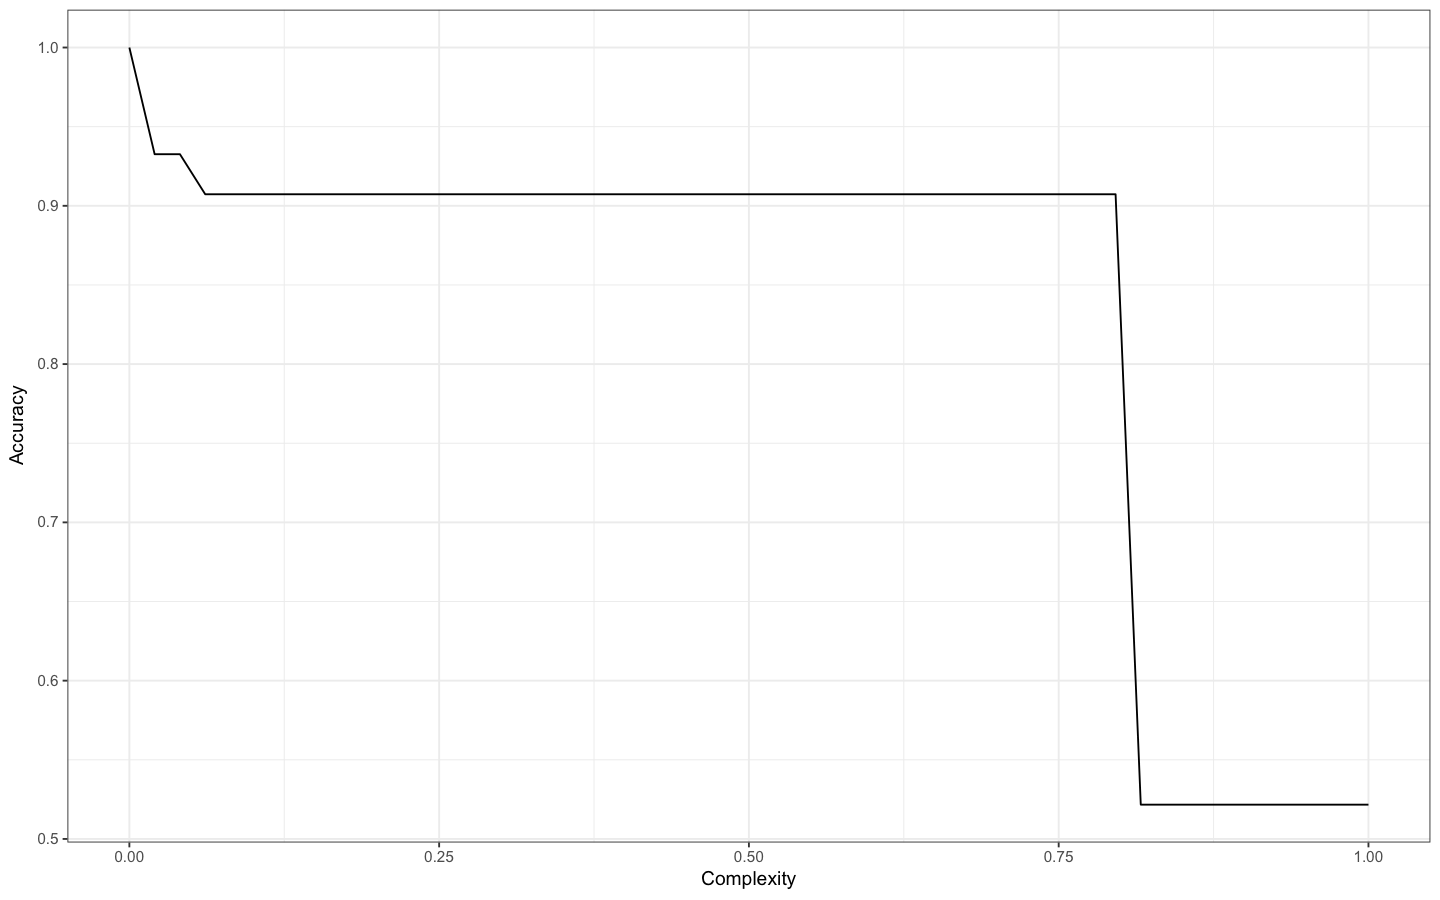
\includegraphics[scale=0.2]{search.png}
  \centering
  \caption{The accuracy during the grid search on the validation data}
\end{figure}

Surprisingly, with no regularization, we obtained an accuracy of 100\% on the validation set and on the test set. Obviously, this is an high estimation... thus, this result is not usable.  Moreover, the tree is too big to understand what is helpful to classify correctly. Thus, with a complexity $\reg=0.1$ we obtained the tree showed in Figure ~\ref{fig:tree}.

\begin{figure}[!hb]
  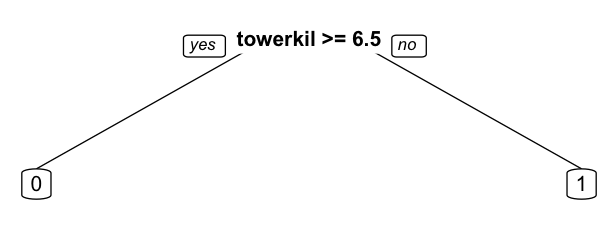
\includegraphics[scale=0.5]{tree.png}
  \centering
  \caption{The tree obtained with $\reg=0.1$}
  \label{fig:tree}
\end{figure}

When we look at the tree, we can notice that this is not the total damage of the champions which split the best. For a decision tree, splitting with the number of tower kills is a good choice. Actually, it can make sense because generally the more towers we destroyed the nearer we are to the enemy base. Moreover, this is a important rule because the tree works well at test time: there are 90.31\% of accuracy. Actually, when we look at the correlation matrix in Figure~\ref{fig:cor1}, the correlation of the outcome and the tower kills is about 0.8 which is a good correlation.

\begin{figure}[!hb]
  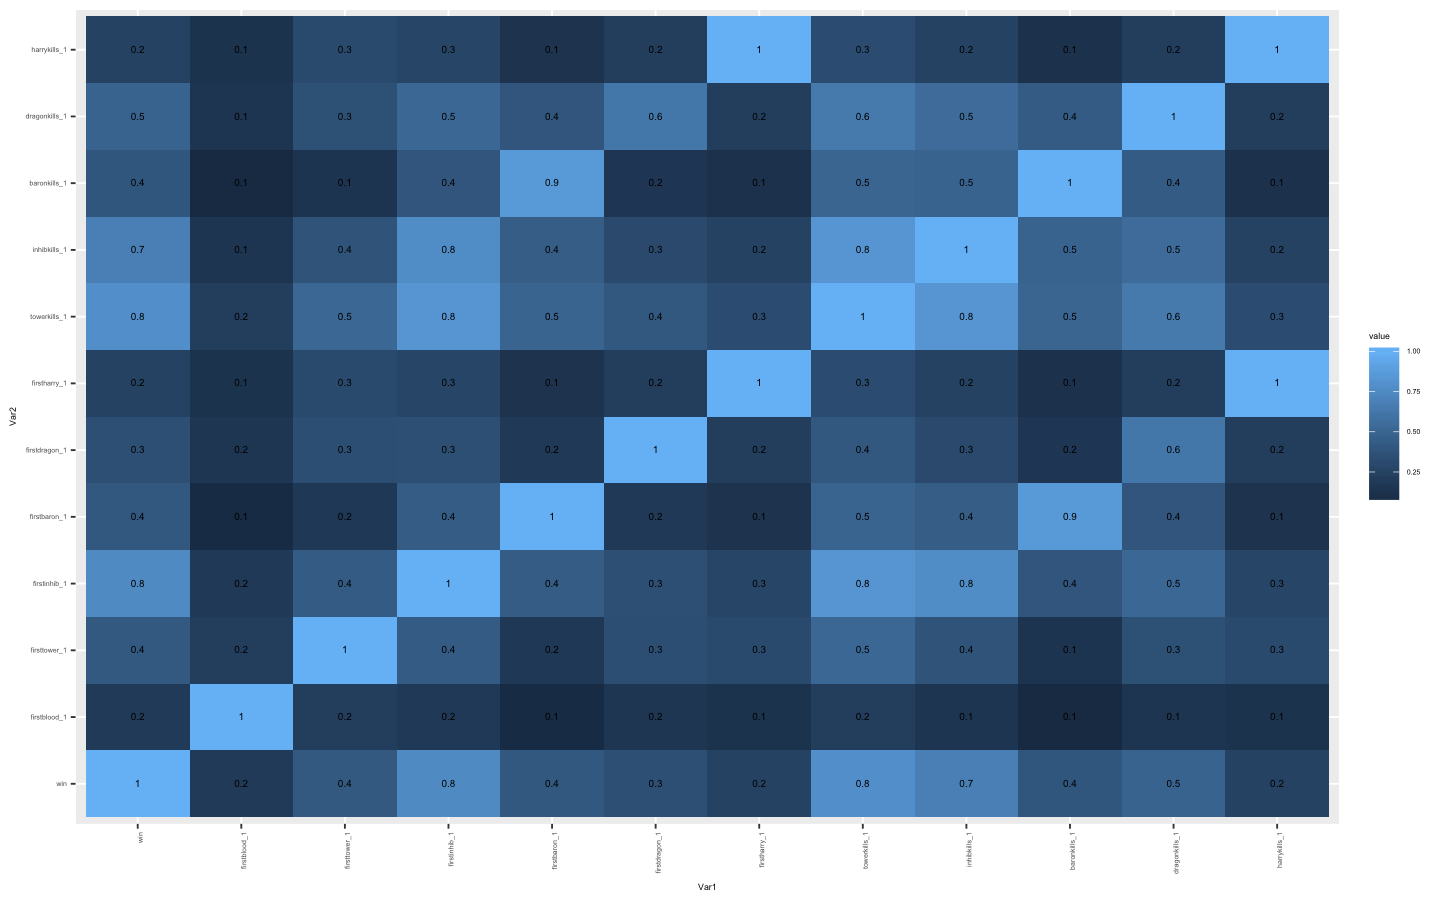
\includegraphics[scale=0.2]{cor1.png}
  \centering
  \caption{The correlation matrix of the table \emph{teamstats} which is stored in $x_{\mathcal{T}1}$}
  \label{fig:cor1}
\end{figure}

Likewise, we obtained the same results with the tree inferred with the gini index using the grid search.

Finally, we inferred a random forest which has good results. After testing manually (due to the time it takes to compute the model), the best parameter for the number of trees was 50. Random forest was one of our best model with an accuracy of 98.19\% with the test data. Moreover, we plotted the importance of the feature i.e we printed the 20 best features where the decrease in Gini index is the most important in average. In the Figure~\ref{fig:importance}, we can notice that the results are consistent with the simple tree: the most important feature is the tower kills and the features which are related to. 

\subsection{Inferring neural networks}

The main drawback of these techniques is that we can't interpret the result of neural networks. But we can still have a good accuracy at test time. We used Keras\footnote{\url{https://keras.rstudio.com}} in R to learn how to predict the outcome with neural networks. First of all, we created a simple feedforward network:

\begin{align*}
z^{1} &= W^{1}x+b^{1}\\
a^{1} &= relu(z^{1})\\
z^{2} &= W^{2}x+b^{2}\\
a^{2} &= relu(z^{2})\\
z^{3} &= W^{3}x+b^{3}\\
y &= softmax(z^{3})\\
\end{align*}

The model was trained with 10 epoch and with Adam optimizer.
We used an early stopping algorithm to regularize the model: when the accuracy with the validation set increased, we saved the model. At the end, we kept the best model and we had an accuracy of 95.24\% at test time.

We tested another type of neural networks: the Convolutional Neural Network (CNN). Indeed, when we looked at the correlation matrix, we noticed that a lot of variables was highly correlated as we can see in the Figure~\ref{fig:cor2} and giving the fact that a given pixel is highly correlated with its neighbors, we can consider here that an example is a 1 dimensional picture. Thus, we tested the following network:

\begin{verbatim}
    _______________________________________________________
    Layer (type)                        Output Shape
    =======================================================
    reshape_1 (Reshape)                 (None, 463, 1)
    _______________________________________________________
    conv1d_1 (Conv1D)                   (None, 459, 1000) 
    _______________________________________________________
    activation_1 (Activation)           (None, 459, 1000) 
    _______________________________________________________
    average_pooling1d_1 (AveragePooling) (None, 229, 1000)
    _______________________________________________________
    flatten_1 (Flatten)                 (None, 229000)
    _______________________________________________________
    dense_1 (Dense)                     (None, 2)
    _______________________________________________________
    activation_2 (Activation)           (None, 2) 
    =======================================================
\end{verbatim}
This model is slightly the same as before we just use one convolution instead of using fully connected neurons. We reach an accuracy of 97.50\% at test time.

\section{Conclusion}
To predict the outcome of the game we can use the random forest: the majority vote makes the forest robust for the prediction. Furthermore, if we want an hint for the beginning of the match, we can use the basket analysis to see who is the champion to avoid.

\section{Appendix}
\begin{sidewaysfigure}[ht]
    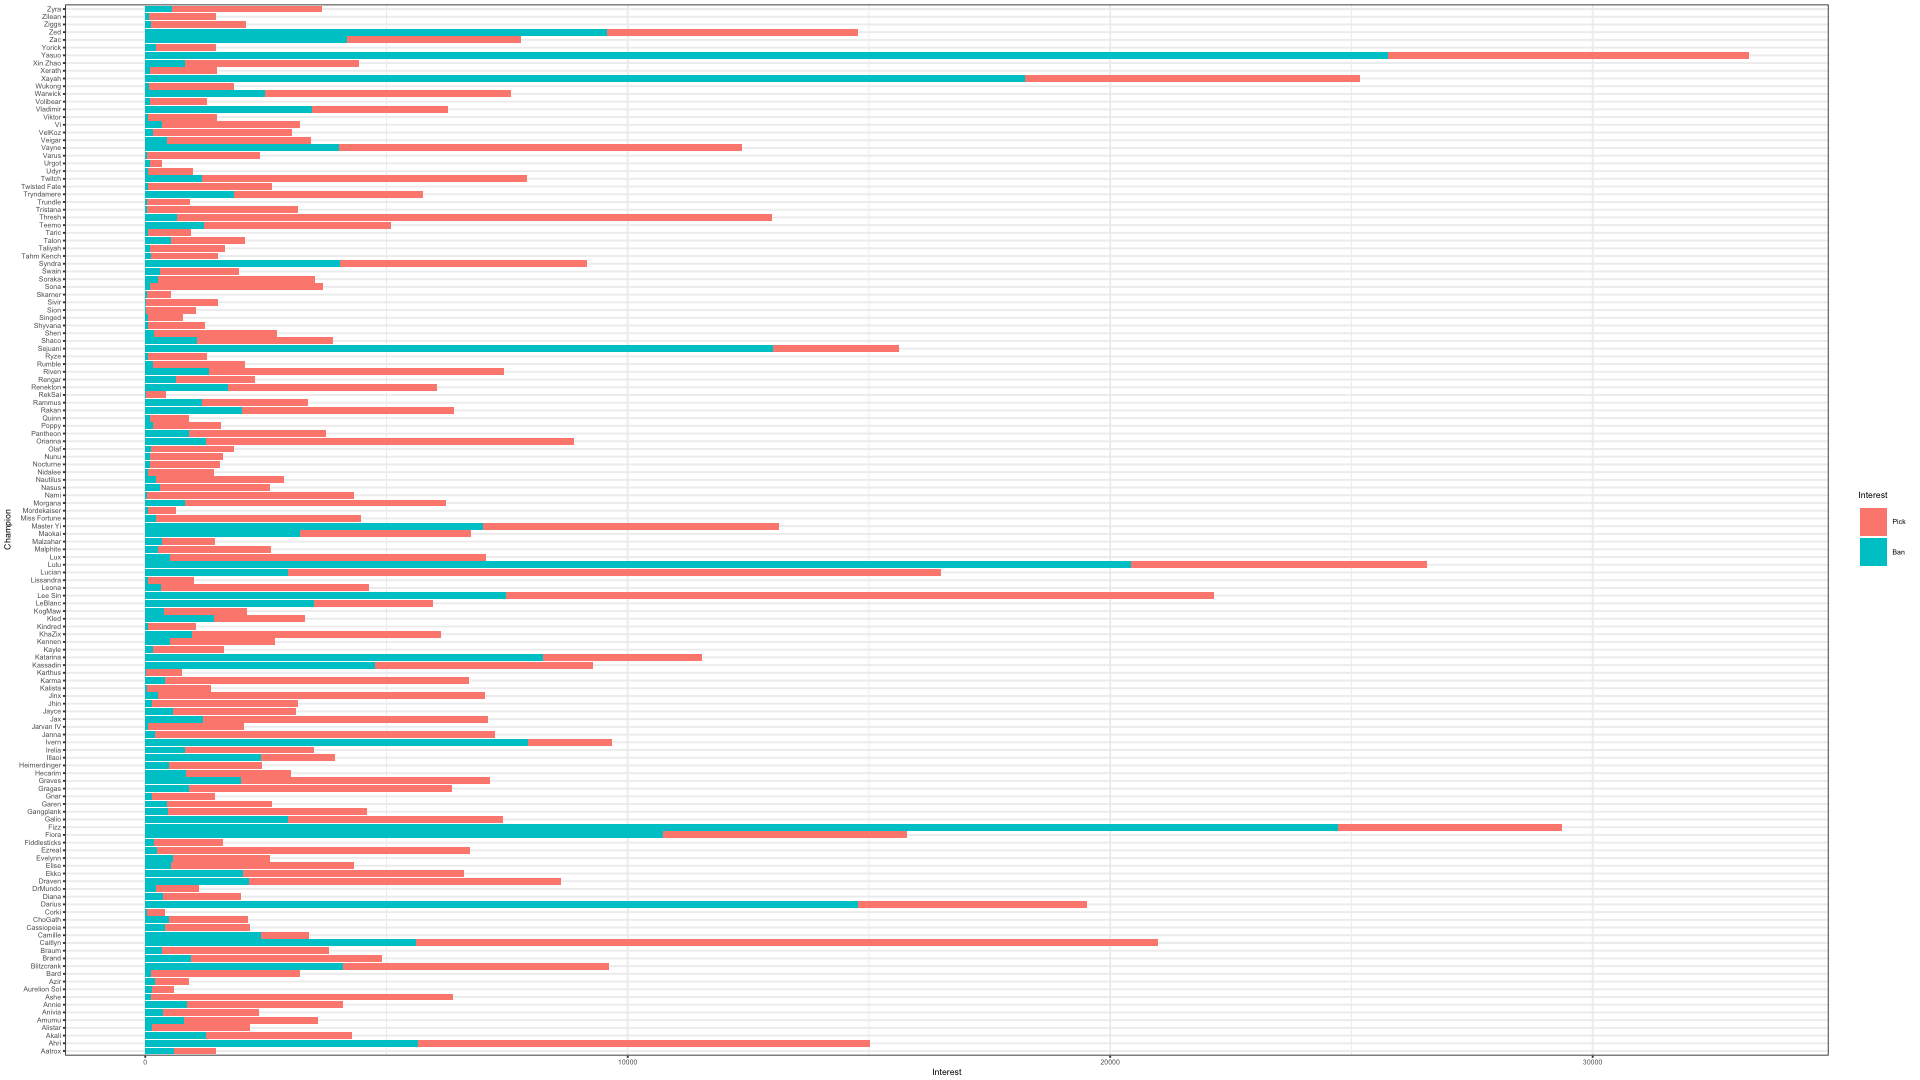
\includegraphics[scale=0.35]{freq.png}
    \caption{The interest for each champions}
    \label{fig:freq}
\end{sidewaysfigure}

\begin{sidewaysfigure}[ht]
    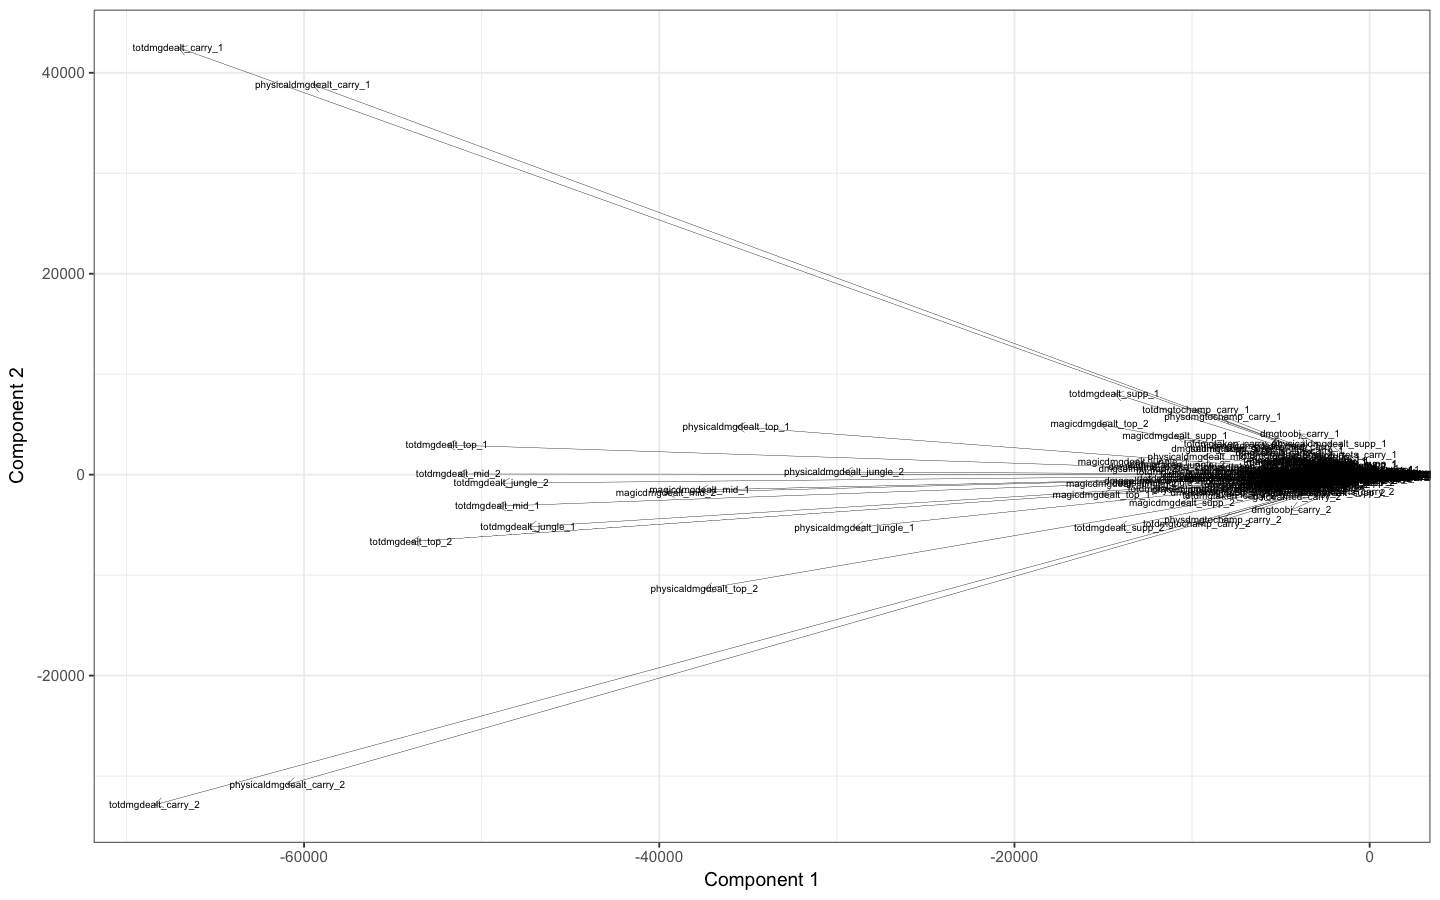
\includegraphics[scale=0.45]{vectors.png}
    \caption{The vectors of the old space projected in 2D}
    \label{fig:vectors}
\end{sidewaysfigure}

\begin{sidewaysfigure}[ht]
    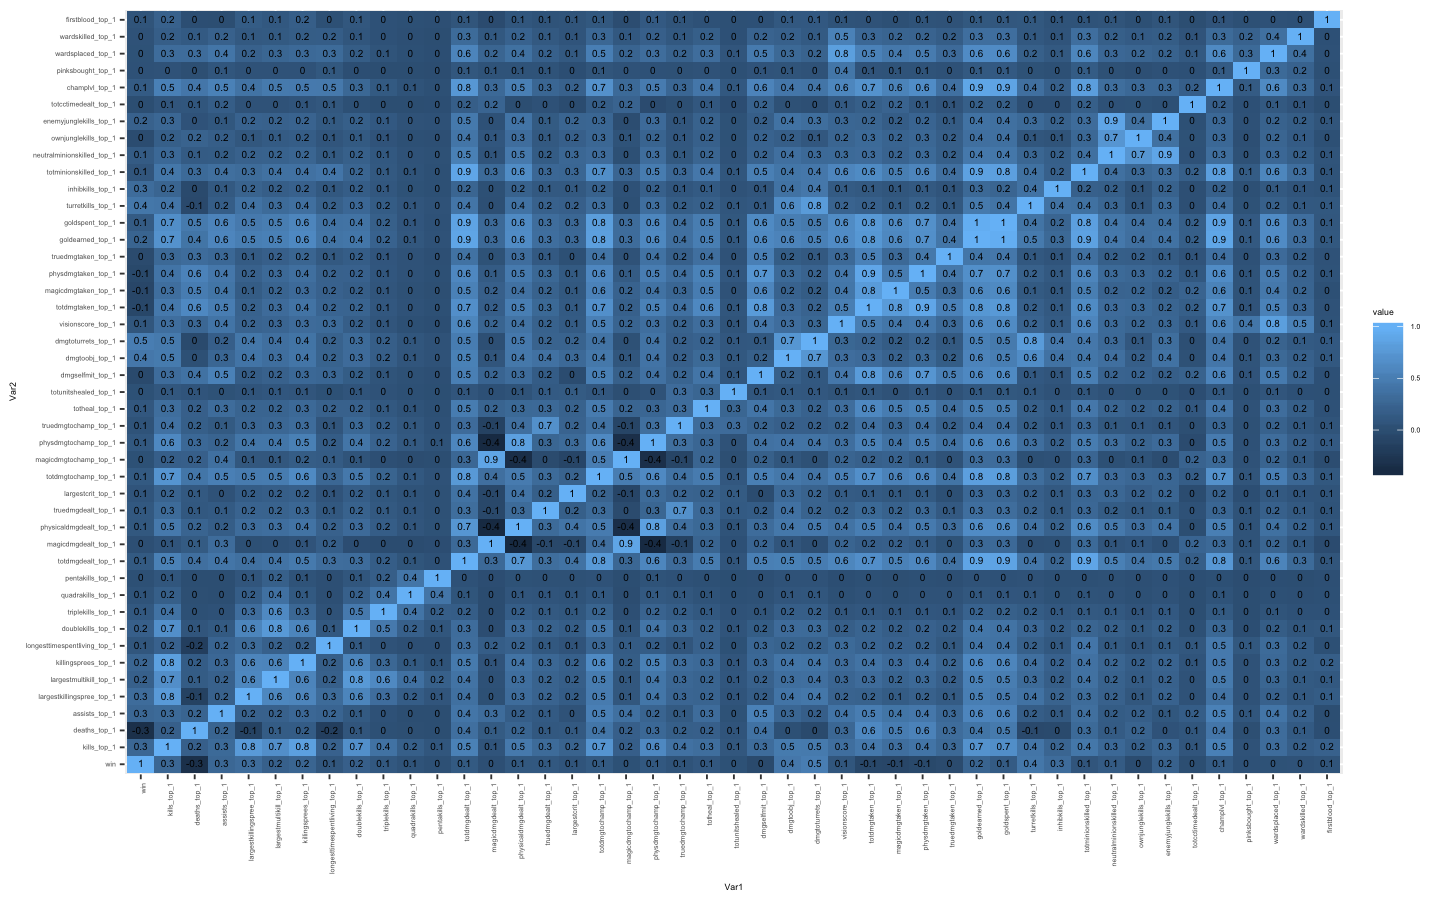
\includegraphics[scale=0.45]{cor2.png}
    \caption{The correlation matrix of the table \emph{stats} for the role top which is stored in $x_{\mathcal{T}1}$}
    \label{fig:cor2}
\end{sidewaysfigure}

\begin{sidewaysfigure}[ht]
    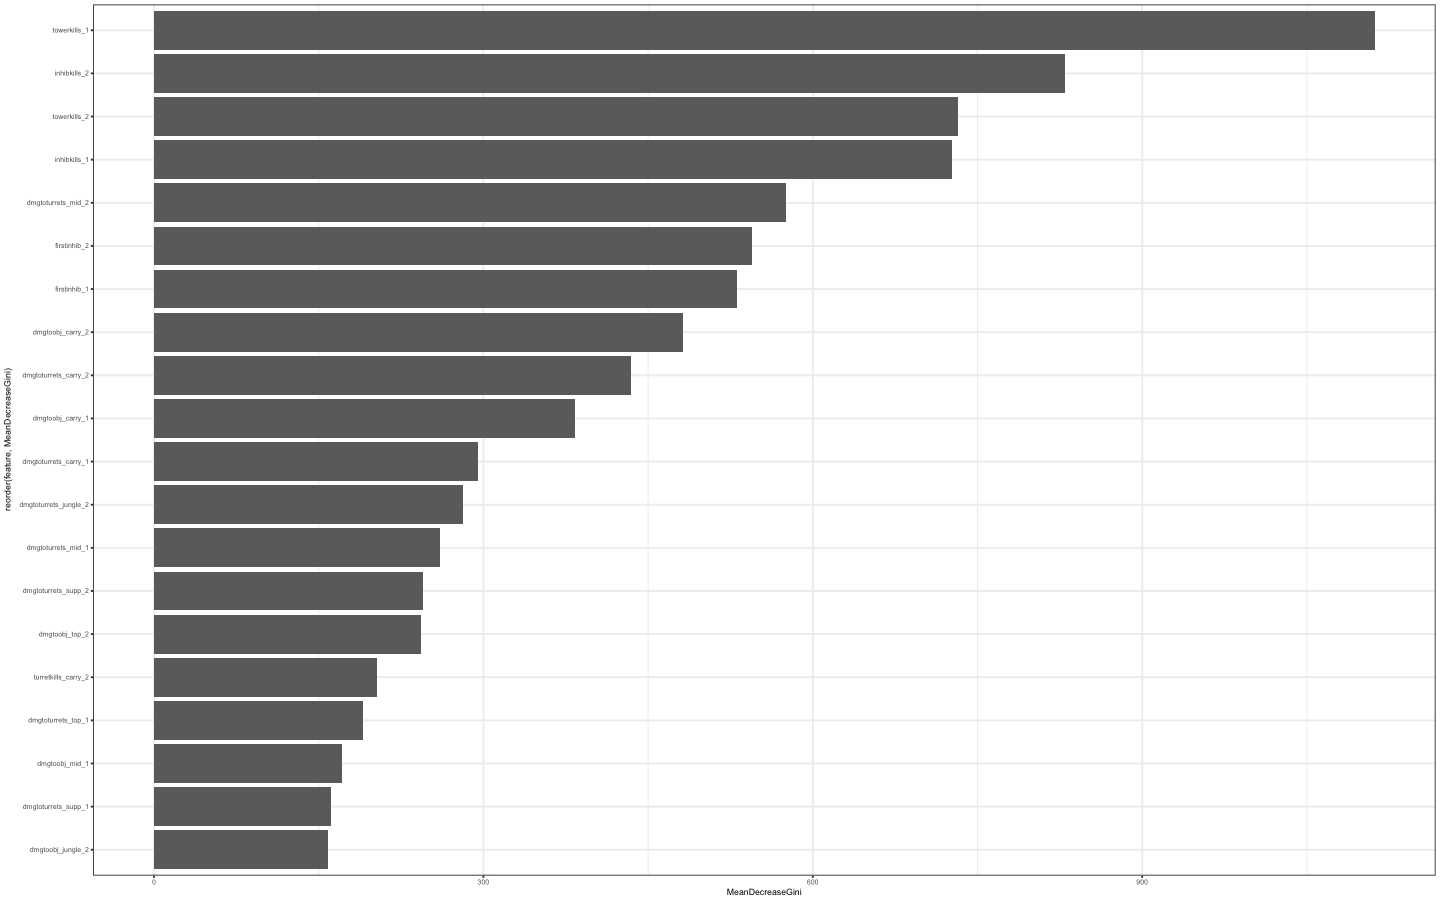
\includegraphics[scale=0.45]{importance.png}
    \caption{The 20 best important features}
    \label{fig:importance}
\end{sidewaysfigure}

\end{document}
